%%%%%%%%%%%%%%%%%%%%%%%%%%%%%%%%%%%
%This is the LaTeX ARTICLE template for RSC journals
%Copyright The Royal Society of Chemistry 2016
%%%%%%%%%%%%%%%%%%%%%%%%%%%%%%%%%%%

\documentclass[twoside,twocolumn,9pt]{article}
\usepackage{extsizes}
\usepackage[super,sort&compress,comma]{natbib} 
\usepackage[version=3]{mhchem}
\usepackage[left=1.5cm, right=1.5cm, top=1.785cm, bottom=2.0cm]{geometry}
\usepackage{balance}
\usepackage{times,mathptmx}
\usepackage{sectsty}
\usepackage{graphicx} 
\usepackage{lastpage}
\usepackage[format=plain,justification=justified,singlelinecheck=false,font={stretch=1.125,small,sf},labelfont=bf,labelsep=space]{caption}
\usepackage{float}
\usepackage{fancyhdr}
\usepackage{fnpos}
\usepackage[english]{babel}
\usepackage{amsmath}
\addto{\captionsenglish}{%
  \renewcommand{\refname}{Notes and references}
}
\usepackage{array}
\usepackage{droidsans}
\usepackage{charter}
\usepackage[T1]{fontenc}
\usepackage[usenames,dvipsnames]{xcolor}
\usepackage{setspace}
\usepackage[compact]{titlesec}
\usepackage{hyperref}
%%%Please don't disable any packages in the preamble, as this may cause the template to display incorrectly.%%%

\newcommand*{\citen}[1]{%
	\begingroup
	\romannumeral-`\x % remove space at the beginning of \setcitestyle
	\setcitestyle{numbers}%
	\cite{#1}%
	\endgroup   
}

\usepackage{epstopdf}%This line makes .eps figures into .pdf - please comment out if not required.

\definecolor{cream}{RGB}{222,217,201}

\begin{document}

\pagestyle{fancy}
\thispagestyle{plain}
\fancypagestyle{plain}{

%%%HEADER%%%
\fancyhead[C]{
\includegraphics[width=18.5cm]{head_foot/header_bar}}
\fancyhead[L]{\hspace{0cm}\vspace{1.5cm}
\includegraphics[height=30pt]{head_foot/journal_name}}
\fancyhead[R]{\hspace{0cm}\vspace{1.7cm}
\includegraphics[height=55pt]{head_foot/RSC_LOGO_CMYK}}
\renewcommand{\headrulewidth}{0pt}
}
%%%END OF HEADER%%%

%%%PAGE SETUP - Please do not change any commands within this section%%%
\makeFNbottom
\makeatletter
\renewcommand\LARGE{\@setfontsize\LARGE{15pt}{17}}
\renewcommand\Large{\@setfontsize\Large{12pt}{14}}
\renewcommand\large{\@setfontsize\large{10pt}{12}}
\renewcommand\footnotesize{\@setfontsize\footnotesize{7pt}{10}}
\makeatother

\renewcommand{\thefootnote}{\fnsymbol{footnote}}
\renewcommand\footnoterule{\vspace*{1pt}% 
\color{cream}\hrule width 3.5in height 0.4pt \color{black}\vspace*{5pt}} 
\setcounter{secnumdepth}{5}

\makeatletter 
\renewcommand\@biblabel[1]{#1}            
\renewcommand\@makefntext[1]% 
{\noindent\makebox[0pt][r]{\@thefnmark\,}#1}
\makeatother 
\renewcommand{\figurename}{\small{Fig.}~}
\sectionfont{\sffamily\Large}
\subsectionfont{\normalsize}
\subsubsectionfont{\bf}
\setstretch{1.125} %In particular, please do not alter this line.
\setlength{\skip\footins}{0.8cm}
\setlength{\footnotesep}{0.25cm}
\setlength{\jot}{10pt}
\titlespacing*{\section}{0pt}{4pt}{4pt}
\titlespacing*{\subsection}{0pt}{15pt}{1pt}
%%%END OF PAGE SETUP%%%

%%%FOOTER%%%
\fancyfoot{}
\fancyfoot[LO,RE]{\vspace{-7.1pt}
\includegraphics[height=9pt]{head_foot/LF}}
\fancyfoot[CO]{\vspace{-7.1pt}\hspace{13.2cm}
\includegraphics{head_foot/RF}}
\fancyfoot[CE]{\vspace{-7.2pt}\hspace{-14.2cm}
\includegraphics{head_foot/RF}}
\fancyfoot[RO]{\footnotesize{\sffamily{1--\pageref{LastPage} ~\textbar  \hspace{2pt}\thepage}}}
\fancyfoot[LE]{\footnotesize{\sffamily{\thepage~\textbar\hspace{3.45cm} 1--\pageref{LastPage}}}}
\fancyhead{}
\renewcommand{\headrulewidth}{0pt} 
\renewcommand{\footrulewidth}{0pt}
\setlength{\arrayrulewidth}{1pt}
\setlength{\columnsep}{6.5mm}
\setlength\bibsep{1pt}
%%%END OF FOOTER%%%

%%%FIGURE SETUP - please do not change any commands within this section%%%
\makeatletter 
\newlength{\figrulesep} 
\setlength{\figrulesep}{0.5\textfloatsep} 

\newcommand{\topfigrule}{\vspace*{-1pt}% 
\noindent{\color{cream}\rule[-\figrulesep]{\columnwidth}{1.5pt}} }

\newcommand{\botfigrule}{\vspace*{-2pt}% 
\noindent{\color{cream}\rule[\figrulesep]{\columnwidth}{1.5pt}} }

\newcommand{\dblfigrule}{\vspace*{-1pt}% 
\noindent{\color{cream}\rule[-\figrulesep]{\textwidth}{1.5pt}} }

\makeatother
%%%END OF FIGURE SETUP%%%

%%%TITLE, AUTHORS AND ABSTRACT%%%
\twocolumn[
  \begin{@twocolumnfalse}
\vspace{3cm}
\sffamily
\begin{tabular}{m{4.5cm} p{13.5cm} }


\includegraphics{head_foot/DOI} & \noindent\LARGE{\textbf{Probabilistic determination of the effect of a deep-eutectic solvent on the structure of lipid monolayers}} \\%Article title goes here instead of the text "This is the title"
\vspace{0.3cm} & \vspace{0.3cm} \\

 & \noindent\large{Adrian Sanchez-Fernandez,\textit{$^{ab}$}$^{\dag\P}$ Andrew R. McCluskey,\textit{$^{ac}$}$^{\dag}$ Karen J. Edler,\textit{$^{a}$}$^{\ast}$ Andrew J. Jackson,\textit{$^{bd}$} Richard A. Campbell,\textit{$^{e}$} and Thomas Arnold\textit{$^{abc}$}} \\%Author names go here instead of "Full name", etc.


\includegraphics{head_foot/dates} & \noindent\normalsize{Deep eutectic solvents present a novel class of non-aqueous room temperature solvent, with tunable properties and capable of promoting self-assembly of surfactant molecules. However, the interactions between the deep eutectic solvent and the surface-active compounds is not well understood. In this work, we present the first example of the self-assembly of a phospholipid monolayer at the interface between air and a non-aqueous solvent. Furthermore, we use novel, chemically-relevant modelling of reflectometry measurements to show the ability for the deep eutectic solvent to have an interaction with the phosphocholine lipid head group, leading to an apparent reduction in the component volume compared to that observed in water. No such reduction was observed for the phosphatidylglycerol head group, indicating that the interaction is ion specific.} \\

\end{tabular}

	\end{@twocolumnfalse} \vspace{0.6cm}

  ]
%%%END OF TITLE, AUTHORS AND ABSTRACT%%%

%%%FONT SETUP - please do not change any commands within this section
\renewcommand*\rmdefault{bch}\normalfont\upshape
\rmfamily
\section*{}
\vspace{-1cm}


%%%FOOTNOTES%%%

\footnotetext{\textit{$^{a}$~Department of Chemistry, University of Bath, Claverton Down, Bath, BA2 7AY, UK.}}
\footnotetext{\textit{$^{b}$~European Spallation Source, SE-211 00 Lund, Sweden.}}
\footnotetext{\textit{$^{c}$~Diamond Light Source, Harwell Campus, Didcot, OX11 0DE, UK.}}
\footnotetext{\textit{$^{d}$~Department of Physical Chemistry, Lund University, SE-211 00 Lund, Sweden.}}
\footnotetext{\textit{$^{e}$~Institut Laue-Langevin, 71 avenue des Martyrs, 38000, Grenoble, France.}}
\footnotetext{\textit{$^{\P}$~Present address: Department of Food Technology, Lund University, SE-211 00 Lund, Sweden}}
\footnotetext{$^{\ast}$~Corresponding author: k.edler@bath.ac.uk}


%Please use \dag to cite the ESI in the main text of the article.
%If you article does not have ESI please remove the the \dag symbol from the title and the footnotetext below.
\footnotetext{\dag~Electronic Supplementary Information (ESI) available: A series Jupyter notebooks and Python plotting scripts, allowing for a fully reproducible analysis of all data presented herein as well as figures showing the probability distribution functions for each of the lipid models. See DOI: 10.1039/b000000x/}
%additional addresses can be cited as above using the lower-case letters, c, d, e... If all authors are from the same address, no letter is required

\footnotetext{$^{\dag}$~These authors have contributed equally to the work presented within.}
%\footnotetext{\ddag~Additional footnotes to the title and authors can be included \textit{e.g.}\ `Present address:' or `These authors contributed equally to this work' as above using the symbols: \ddag, \textsection, and \P. Please place the appropriate symbol next to the author's name and include a \texttt{\textbackslash footnotetext} entry in the the correct place in the list.}


%%%END OF FOOTNOTES%%%

%%%MAIN TEXT%%%%
\section{Introduction}
Deep eutectic solvents (DES) are green, sustainable solvents obtained through the complexation of naturally occurring compounds, such as sugars, alcohols, amines and carboxylic acids, amoung others.\cite{Smith2014, Dai2013} An extensive hydrogen-bonding network is present between these precursors, allowing the mixture to remain liquid at room temperature due to the high-entropic state of the mixture.\cite{Hammond2016, Hammond2017, Araujo2017} Additionally, through different combinations of the precursors materials, it is possible to tune the physicochemical properties of the solvent, such as polarity,\cite{Pandey2014} viscosity and surface tension,\cite{Smith2014} network charge,\cite{Zahn2016} and hydrophobicity.\cite{Ribeiro2015,vanOsch2015} 

These solvents have recently shown the ability to promote the self-assembly of surfactants into micellar structures\cite{Sanchez-Fernandez2016,Arnold2015} and to stabilise the conformation of non-ionic polymer species,\cite{Sapir2016} indicating the presense of a solvophobic effect. The behaviour and conformation of biomolecules in DES has seen and increase in interest,\cite{Esquembre2013,Gorke2010,Gorke2008,Monhami2014,Wu2014,Harifi-Mood2017,Milano2017,Sanchez-Fernandez2017} due to potential applications in the preservation of biomolecules, as environments for enzymatic reactions.\cite{Merza2018} Futhermore, recent investigations have also shown that DES have been shown to support the formation of phospholipid bilayers.\cite{Bryant2017,Bryant2016,Gutierrez2009} 

The formation of phospholipid monolayers plays a key role in many biological and technological processes. Amphiphilic lipids commonly show a low soluibilty in the one of the two phases, leading to the formation of a stable monolayer at the interface.\cite{Mohwald1990} Phospholipids consist of a charged headgroup, either anionic or zwitterionic, and investigations at the air-salt water interface have revealed the importance of the lipid-ion interactions on structure, monomer packing, and stability of the monolayer.\cite{Mohwald1990,Kewalramani2010} Despite the broad interest in these systems, the presence of stable phospholipid monolayers in non-aqueous media has not been previously reported, to the best of the authors' knowledge. 

Recent developments in computational resource and software has enabled powerful methodologies and algorithms to be harnessed by those from non-computer science backgrounds. This has mostly occurred through open-source software projects such as the Python language and the Jupyter notebooks framework.\cite{vanRossum1995,Kluyver2016} In the area of neutron and X-ray reflectometry data-analysis, this has led to the development of refnx,\cite{Nelson2018} a Python library for the fitting of layer-based models to reflectometry data. refnx enables the use of custom models that contain chemically-relevant information. This information includes constaints such as that the number density of phospholipid headgroups must be the same as the number density of pairs of phospholipid tailgroups and that the length of the tail chains should be equal to the Tanford length.\cite{Tanford1980}

The use of a Python library for fitting enables powerful probability distribution function (PDF) sampling methods to be used such as the Goodman \& Weare Affine Invariant Markov chain Monte Carlo (MCMC) Ensemble,\cite{Goodman2010} as implemented in the Python library emcee.\cite{Foreman-Mackey2013} This method allows for the sampling of a high-dimensionality parameter space, such as that which is relevant to reflectometry fitting, to be performed with relative ease. This results in estimatations of the inverse uncertainties associated with each parameter as well as information about the correlations between different parameters within the model. 

In this work, we present the first investigation of the structure of phospholipid monolayers at the air-DES interface, as determined by chemical-context modelling of X-ray reflectometry measurements. Four different phospholipids; 1,2-dipalmitoyl-sn-glycero-3-phosphocholine (DPPC), 1,2-dimyristoyl-sn-glycero-3-phosphocholine (DMPC),  1,2-dilauroyl-sn-glycero-3-phosphocholine (DLPC) and 1,2-dimyristoyl-sn-glycero-3-phospho-(1'-rac-glycerol) (DMPG), were studied at the interface between a 1:2 mixture of choline chloride:glycerol and air. This allowed the nature of two, chemically distinct, phospholipid headgroups to be understood in this non-aqueous solvent, in addition to the effect of the tail chain length. 

\section{Experimental}

\subsection{Materials}
Choline chloride (99 \%, Sigma-Aldrich) and glycerol (99 \%, Sigma-Aldrich) were purchased and used without further purification. The DES was prepared by mixing the precursors at the appropriate mole ratio, and heating at 80 $^\circ$C until a homogeneous, transparent liquid formed.\cite{Smith2014} The solvent was equilibrated overnight at 40 $^\circ$C and subsequently stored under a dry atmosphere. 

The water content on the DES was determined before and after each experiment by Karl-Fischer titration (Mettler Toledo DL32 Karl-Fischer Coulometer, Aqualine Electrolyte A, Aqualine Catholyte CG A) in order to ensure water presence was kept to a minimum. Those measurements showed that the water content of the solvent was kept below 0.3 wt\% during all the experimental procedures presented here, which we assume to be negligible and have little impact on the characteristics of the DES.\cite{Hammond2016,Hammond2017}

DPPC (> 99 \%), DMPC (> 99 \%), and DMPG (> 99 \%) were supplied by Avanti Polar Lipids and DLPC (> 99 \%) was supplied by Sigma-Aldrich and all were used as received. Sample preparation was performed in situ using the standard method for the spreading of insoluble monolayers on water: a certain amount of the phospholipid solution was spread onto the liquid surface in order to provide a given surface concentration. After the evaporation of the chloroform, it is assumed that the resulting system is a solvent subphase with a monolayer of phospholipid at the interface. Surface concentration was modified by closing and opening the PTFE barriers of the Langmuir trough.

\subsection{Methods}
X-ray reflectivity measurements were taken on I07 at Diamond Light Source, at 12.5 keV photon energy using the double-crystal-deflector.\cite{Arnold2012} The reflected intensity was measured in a momentum transfer range from 0.018 to 0.7 \AA$^{-1}$. The data was normalised with respect to the incident beam and the background was measured from off-specular reflection and subsequently subtracted. The sample environment consisted of a PTFE Langmuir trough. Samples were equilibrated for at least one hour and preserved under argon atmosphere to minimise the adsorption of water by the subphase. Surface concentration was controlled through opening and closing the barriers of the Langmuir trough. X-ray reflectivity data were collected for each of the lipids, DMPC, DPPC, DLPC and DMPG and all measurements were made at 22 $^\circ$C at five different surface concentrations, however full analysis was only performed for the two highest surface concentrations where the monolayer would be in the condensed phase. 

\subsection{Data analysis}
The use of reflectometry to analyse the structure of phospholipids on the surface of water has a histroy extending over many years.\cite{Mohwald1990,Kewalramani2010,Bayerl1990,Johnson1991,Clifton2012,Helm1987,Daillant1990} This has led to some variation in the models used to fit experimental data, shown in Table \ref{tab:water}. Although, there appears to be a general consensus that the volume of the phosphocholine is in the range from 320 \AA$^3$ to 360 \AA$^3$, and as a result this volume is often used as a physical constraint on the layer model when fitting reflectometry data. However, this work involves the use of a non-aqueous solvent system and we believe that the these literature values for the head group volumes may be unreliable in such media. This is due to the charged nature of the zwitterionic and anionic lipid heads having a significant interaction with the solvent in both the neutral water and the charged DES. 

\begin{table*}
	\small
	\caption{\ Lipid component volumes extracted from different literature sources. $V_l$ corresponds to the total lipid volume, MD to molecular dynamics simulation, WAXS to wide-angle X-ray scattering, NB to neutral buoyancy and DVTS to differential vibrating tube densimetry}
	\label{tab:water}
	\begin{tabular*}{\textwidth}{@{\extracolsep{\fill}}lllllllll}
		\hline 
		Lipid & DPPC & & & & DMPC & & & DMPG \\
		\hline
		Reference & [\citen{Armen1998}] & [\citen{Petrache1997}] & [\citen{Sun1994}] & [\citen{Tardieu1973}] & [\citen{Kucerka2004}] & [\citen{Nagle1978}] & [\citen{Schmidt1985}] & [\citen{Pan2012}] \\
		$V_l$/\AA$^3$ &1216.96 & 1219 & 1148 & 1224 & 1101 & 1061 & 1094 & 1058 \\
		$V_h$/\AA$^3$ & 326.00 & 324 & 319 & 360 & 319 & 344 & & 291 \\
		$V_t$/\AA$^3$ & 890.96 & 895 & 829 & 864 & 782 & 717 & & 767 \\
		Method & MD & MD & WAXS & NB & NB & NB & DVTS & DVTS \\
		T/$^\circ$C & 25 & 50 & 24 & 25 & 30 & 30 & & 30 \\
		\hline
	\end{tabular*}
\end{table*}

To allow for the use of a chemically-relevant model, where the lipid head group volume was allowed to vary, the Python library refnx\cite{Nelson2018} as used. This software allows the inclusion of a custom chemically-relevant model from which the parameters to be fed into the Abel\`{e}s layer-model,\cite{Abeles1950,Parratt1954} that is typical for reflectometry fitting, are obtained. This custom model, along with Jupyter notebook showing in full the analysis performed, can be found in the ESI. 

This chemically-relevant model involves considering the lipids as consisting of head groups and tail groups. The head groups have a calculated scattering length, $b_h$, (found as a summation of the number of electrons in the head group multiplied by the classical radius of the electron), and a volume, $V_h$. These head groups make up a layer with a given thickness, $d_h$, and roughness, $\sigma_h$, within which some volume fraction of solvent can intercalate, $\phi_h$. The tail groups also have a calculated scattering length, $b_t$, and a volume, $V_t$, however the thickness of the tail group layer, $d_t$, is found from the length of the carbon tail, $t_t$, and angle that the chain is tilted by with respect to the interface normal, $\theta_t$, 
\begin{equation}
\label{equ:tl}
d_t = t_t \cos{\theta_t}.
\end{equation}
The air above the monolayer is also able to solvate the tail region by some volume fraction, $\phi_t$. The scattering length density of the tail and head layers used in the Abel\`{e}s model can therefore be found as follows, 
\begin{equation}
\text{SLD}_i = \frac{b_i}{V_i}(1 - \phi_i) + \text{SLD}_{s}\phi_i,
\end{equation}
where $\text{SLD}_{s}$ is the scattering length density of the superphase (air) and the subphase (DES) for the tail and head groups respectively, and $i$ indicates either the tail or head layer. In order to ensure that the number density of head groups and pairs of tail groups is the same, the following constraint was added to the model,
\begin{equation}
\label{equ:ht}
d_h = \frac{V_hd_t(1-\phi_t)}{V_t(1-\phi_h)}. 
\end{equation}

This custom model was used to co-refine the volume of the lipid head group, $V_h$, for the two highest surface concentration measurements. Other parameters that were allowed to very were $\theta_t$, $\phi_t$, $\phi_h$, $\sigma_t$, and $\sigma_h$, while the parameters shown in Table \ref{tab:invariant} were held constant at the values given. The length of the carbon chain was kept constant to the value determined by the Tanford equation,\cite{Tanford1980} this is valid due to the condensed nature of the monolayer at this surface concentration resulting in the extended, staggered conformation of the chain being likely. 

\begin{table}[h]
	\small
	\caption{\ The variant parameters within the chemically-sensible model. $^a$Values determined from Armen \emph{et al.}\cite{Armen1998} $^b$Values obtained from the Tanford formula where the carbon chains are assumed to be fully extended.\cite{Tanford1980} $^c$Values extracted from Sanchez-Fernandez \emph{et al.}\cite{Sanchez-Fernandez2016}}
	\label{tab:invariant}
	\begin{tabular*}{0.48\textwidth}{@{\extracolsep{\fill}}ll}
		\hline
		Parameter & Value \\
		\hline
		DP-$b_t$/fm & 6897 \\
		DM-$b_t$/fm & 5985 \\
		DL-$b_t$/fm & 5073 \\
		PC-$b_h$/fm & 4674 \\
		PG-$b_h$/fm & 4731 \\
		DP-$V_t$/\AA$^3$ & 891$^a$ \\
		DM-$V_t$/\AA$^3$ & 779$^a$ \\
		DL-$V_t$/\AA$^3$ & 667$^a$ \\	
		DP-$t_t$/\AA & 21.8$^b$ \\
		DM-$t_t$/\AA & 19.3$^b$ \\
		DL-$t_t$/\AA & 16.7$^b$ \\
		$\text{SLD}_{\text{sup}}$/$\times10^{-6}$\AA$^{-2}$ & 0\\
		$\text{SLD}_{\text{sub}}$/$\times10^{-6}$\AA$^{-2}$ & 10.8$^c$ \\
		\hline
	\end{tabular*}
\end{table}

The fitting of the reflectometry model to the experimental involved transforming the reflectometry calculated from the model and the data into $Rq^4$ such that the artifact of the Fresnel decay was removed, before using the differential evoulation method available to refnx from the scipy library,\cite{Jones2001} to find the parameters that gave the best fit to the data. The parameter space was then probed using the MCMC method available through emcee, this allowed for an estimate of the PDF associated with each parameter. In the MCMC sampling, 200 walkers were used over 1000 iterations, following an equilibration of 200 iterations.

\section{Results \& Discussion}

\begin{figure}
	\centering
	
\includegraphics[width=0.48\textwidth]{figures/DLPC_all_data}
	
\includegraphics[width=0.48\textwidth]{figures/DMPC_all_data}
	
\includegraphics[width=0.48\textwidth]{figures/DPPC_all_data}
	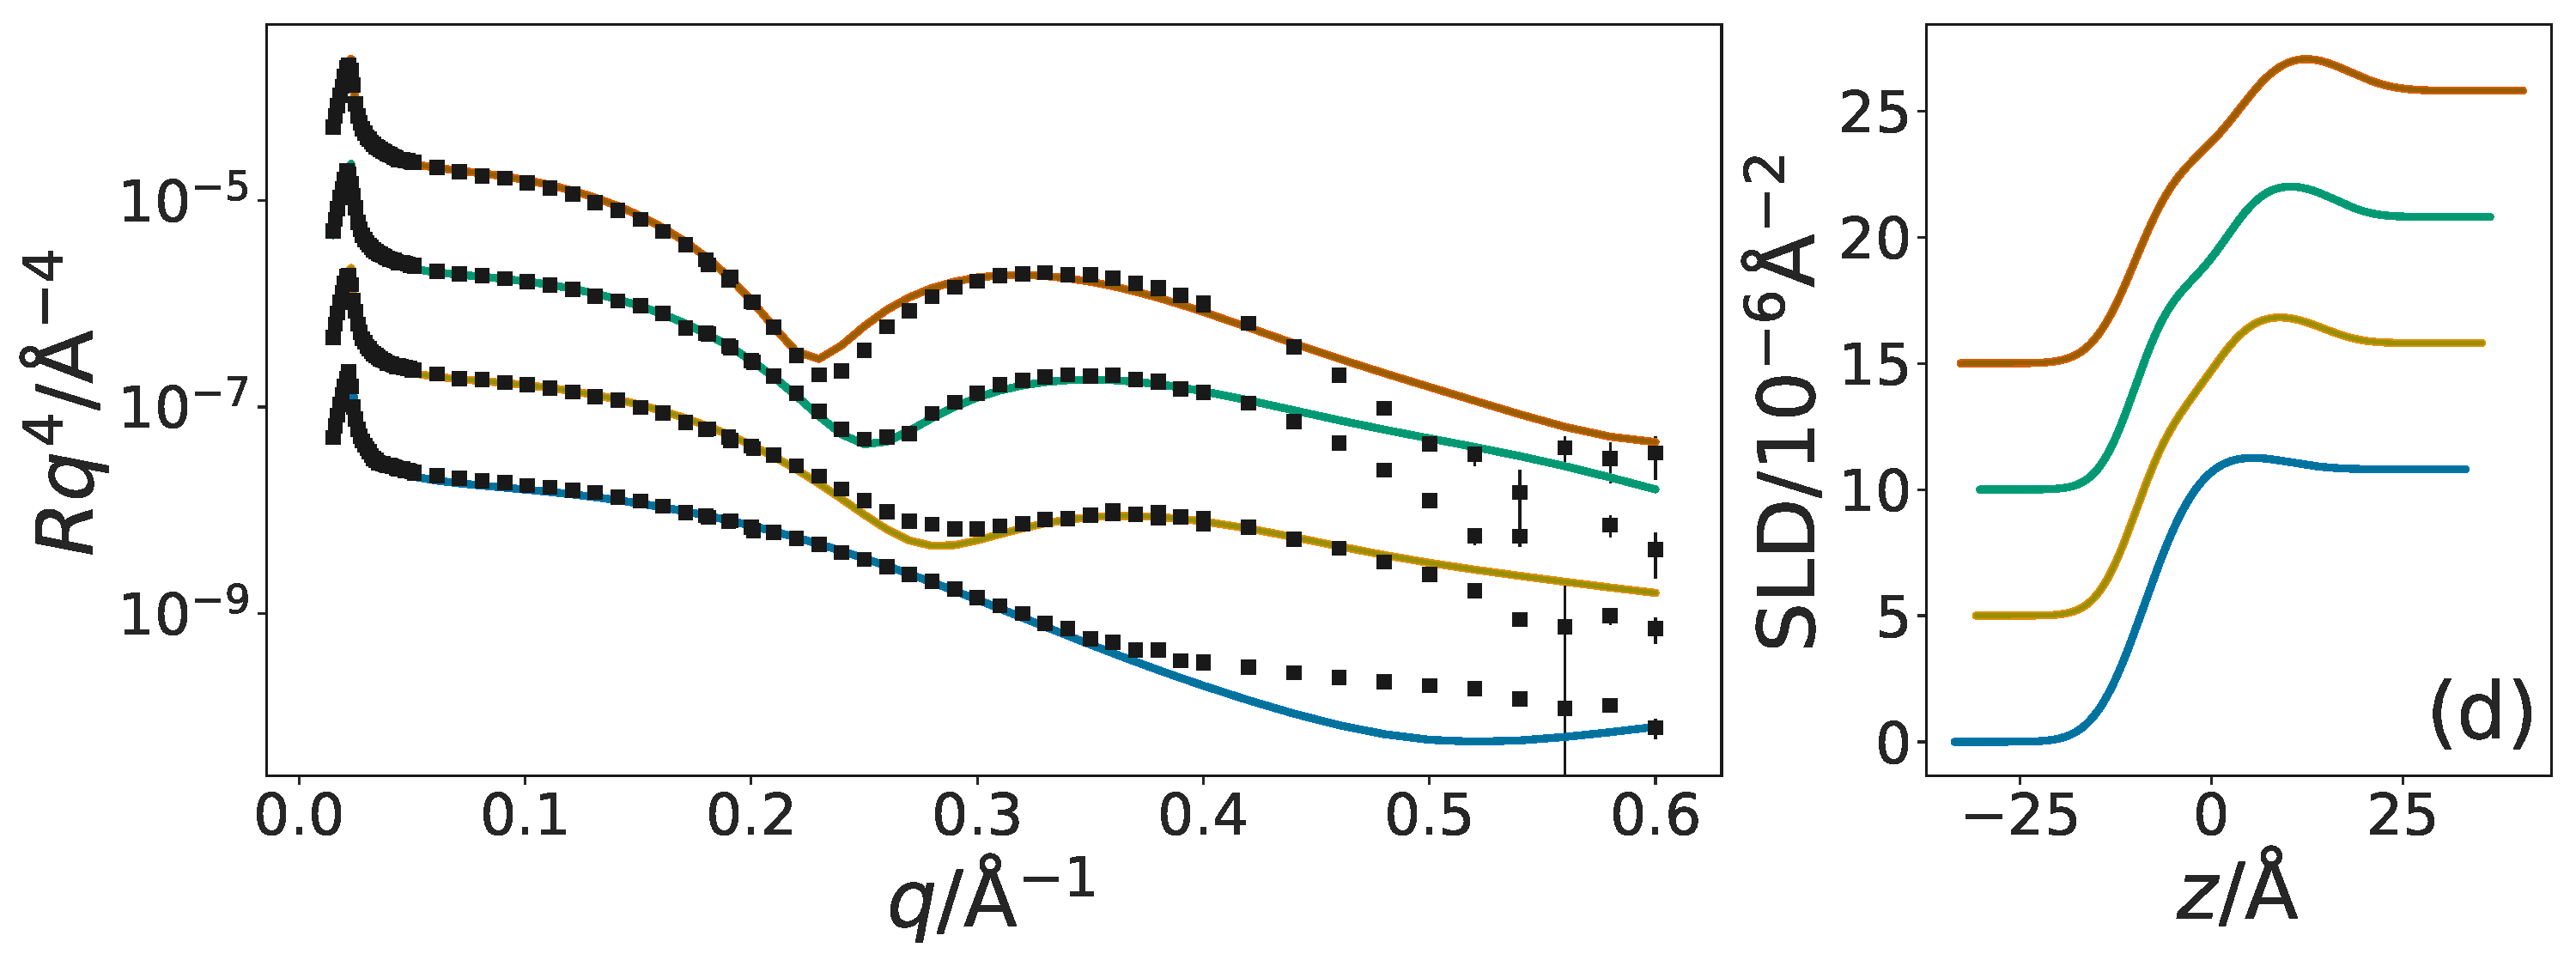
\includegraphics[width=0.48\textwidth]{figures/DMPG_all_data}
	\caption{The reflectometry profile, scattering length density profile and probability distribution function for each of the three phosphocholine containing lipids, the lower surface concentration is shown in blue while the higher in green; (a) DLPC, (b) DMPC, (c) DPPC, (d) DMPG. The reflectometry and SLD profiles have been offset in the $y$-axis for clarity. Figure files are available under MIT License.\cite{mccluskey_2018}}
	\label{fig:lipids}
\end{figure}
The custom model was co-refined for the highest two concentrations of all lipids. The resulting reflectometry profiles, associated scattering length density profiles and the PDF for the head group volume are shown in Figure \ref{fig:lipids}. Table \ref{tab:liptab} gives details of all varying parameters for each lipid, these are given with asymmetric error bars which correspond to a 95 \% confidence interval, the full PDF plots can be found in the ESI. 
\begin{table*}
	\small
	\caption{\ The best-fit values, and associated 95 \% confidence intervals for the varying parameters in the phosphocholine reflectometry model. The values of $d_t$ were found from the appropriate values of $\theta_t$ using Eqn. \ref{equ:tl}. The values of $d_h$ were obtained from the appropriate use of Eqn. \ref{equ:ht}}
	\label{tab:liptab}
	\begin{tabular*}{\textwidth}{@{\extracolsep{\fill}}lllllllll}
		\hline
		 & DLPC & & DMPC & & DPPC & & DMPG & \\
		\hline
		Parameter & Conc 4 & Conc 5 & Conc 4 & Conc 5 & Conc 4 & Conc 5 & Conc 4 & Conc 5 \\
		$\theta_t$/$^\circ$ & \input{../output/dlpc/angle4.txt} & \input{../output/dlpc/angle5.txt} & \input{../output/dmpc/angle4.txt} & \input{../output/dmpc/angle5.txt} & \input{../output/dppc/angle4.txt} & \input{../output/dppc/angle5.txt} & \input{../output/dmpg/angle4.txt} & \input{../output/dmpg/angle5.txt} \\
		$d_t$/\AA & \input{../output/dlpc/tail4.txt} & \input{../output/dlpc/tail5.txt} & \input{../output/dlpc/tail4.txt} & \input{../output/dmpc/tail5.txt} & \input{../output/dppc/tail4.txt} & \input{../output/dppc/tail5.txt} & \input{../output/dmpg/tail4.txt} & \input{../output/dmpg/tail5.txt} \\
		$d_h$/\AA & \input{../output/dlpc/head4.txt} & \input{../output/dlpc/head5.txt} & \input{../output/dlpc/head4.txt} & \input{../output/dmpc/head5.txt} & \input{../output/dppc/head4.txt} & \input{../output/dppc/head5.txt} & \input{../output/dmpg/head4.txt} & \input{../output/dmpg/head5.txt} \\
		$\phi_t$/$\times10^{-2}$ & \input{../output/dlpc/solt4.txt} & \input{../output/dlpc/solt5.txt} & \input{../output/dmpc/solt4.txt} & \input{../output/dmpc/solt5.txt} & \input{../output/dppc/solt4.txt} & \input{../output/dppc/solt5.txt} & \input{../output/dmpg/solt4.txt} & \input{../output/dmpg/solt5.txt} \\
		$\phi_h$/$\times10^{-2}$ & \input{../output/dlpc/solh4.txt} & \input{../output/dlpc/solh5.txt} & \input{../output/dmpc/solh4.txt} & \input{../output/dmpc/solh5.txt} & \input{../output/dppc/solh4.txt} & \input{../output/dppc/solh5.txt} & \input{../output/dmpg/solh4.txt} & \input{../output/dmpg/solh5.txt} \\
		$\sigma_t$/\AA & \input{../output/dlpc/rought4.txt} & \input{../output/dlpc/rought5.txt} & \input{../output/dmpc/rought4.txt} & \input{../output/dmpc/rought5.txt} & \input{../output/dppc/rought4.txt} & \input{../output/dppc/rought5.txt} & \input{../output/dmpg/rought4.txt} & \input{../output/dmpg/rought5.txt} \\
		$\sigma_h$/\AA & \input{../output/dlpc/roughh4.txt} & \input{../output/dlpc/roughh5.txt} & \input{../output/dmpc/roughh4.txt} & \input{../output/dmpc/roughh5.txt} & \input{../output/dppc/roughh4.txt} & \input{../output/dppc/roughh5.txt} & \input{../output/dmpg/roughh4.txt} & \input{../output/dmpg/roughh5.txt} \\
		\hline
	\end{tabular*}
\end{table*}

It can be seen from Table \ref{tab:liptab} that as would be expected, and as found in previous work,\cite{Mohwald1990,Vaknin1991} the thickness of the tail layer increases as the number of carbon atoms in the tail chains increases. Additionally, it is also observed that the value of the chain tilt either decreases, resulting in a tail thickness increase, or remains constant as the surface concentration increases. This indicates that for DLPC and DPPC these two highest surface concentration measurements where at a similar area per molecule, while the area per molecule slightly decreased between the two measurements for DMPC and DPPC. The phenomena of the tail thickness increasing with increasing surface pressure has been note before for DMPC at the air-water interface.\cite{Bayerl1990} Futhermore, as the surface concentration increases, the amount of solvent in the head layer decreases, or stays the same, this would be expected for the head layer becoming more closely-packed and therefore having less space available for solvent. 

The thickness of the tail layers in these condensed monolayers appears to agree well with values found for water-analogues (DMPC: $d_t=15.8$ \AA,\cite{Johnson1991} DPPC: $d_t=16.7$ \AA\cite{Helm1987}). Previous work indicates, although there has been no direct comparison, that the phosphatidylglycerol head layer may be thicker than phosphocholine at a water-air interface.\cite{Clifton2012,Johnson1991,Vaknin1991,Lawrie2000} However, the phosphocholine head group appears to be slightly expanded in the DES compared to in water (DPPC: $d_h=8.4$ \AA\cite{Helm1987}) resulting in the values for the thicknesses of the head layers being similar between the two head groups. 

Figures \ref{fig:lipids}(a-c) show the PDF determined for the head group volume for each of the four lipids. The three lipids with a phosphocholine head group appear to show some small unsystematic variation as the tail length is changed, with values of \input{../output/dlpc/vh.txt} \AA$^{3}$ for DLPC, \input{../output/dmpc/vh.txt} \AA$^{3}$ for DMPC, and \input{../output/dppc/vh.txt} \AA$^{3}$ for DPPC. This is significantly less than the largest estimate of the head volume from literature sources, 360 \AA$^3$,\cite{Tardieu1973} and slightly less than lowest estimate, 319 \AA$^3$.\cite{Sun1994,Kucerka2004} The fact that the choline chloride component of the DES is charged in nature suggests that it may have a screening effect on the charged interactions between the zwitterionic phosphocholine head groups reducing the volume occupied.

Figure \ref{fig:lipids}(d) contains the PDF for the phosphatidylglycerol head group volume, which was found to be \input{../output/dmpg/vh.txt} \AA$^{3}$. This agrees well with the literature value for this lipid head group of 291 \AA$^{3}$,\cite{Pan2012} indictating that the charged component of the DES solvent has little affect on the volume occupied by the phosphatidylglycerol head group. 

It is possible to generalise the difference between the two lipid head groups in terms of the difference in their charges, with the phosphocholine group being zwitterionic in nature while the phosphatidylglycerol is anionic (Figure \ref{fig:heads}). The fact that the phosphatidylglycerol head group appears to show no deviation in volume at the air-DES interface, when compared with the air-water interface, suggests that the interaction resulting in the apparent decrease in volume of the phosphocholine head group is due to the positively-charged nitrogen group interacting with the negatively-charged chlorine component of the DES. The relatively small size of the chloride ion, compared to the choline moiety, means that it is able to intercalate more easily into the lipid head layer allowing for the charge screening to occur. 

\begin{figure}
	\centering
	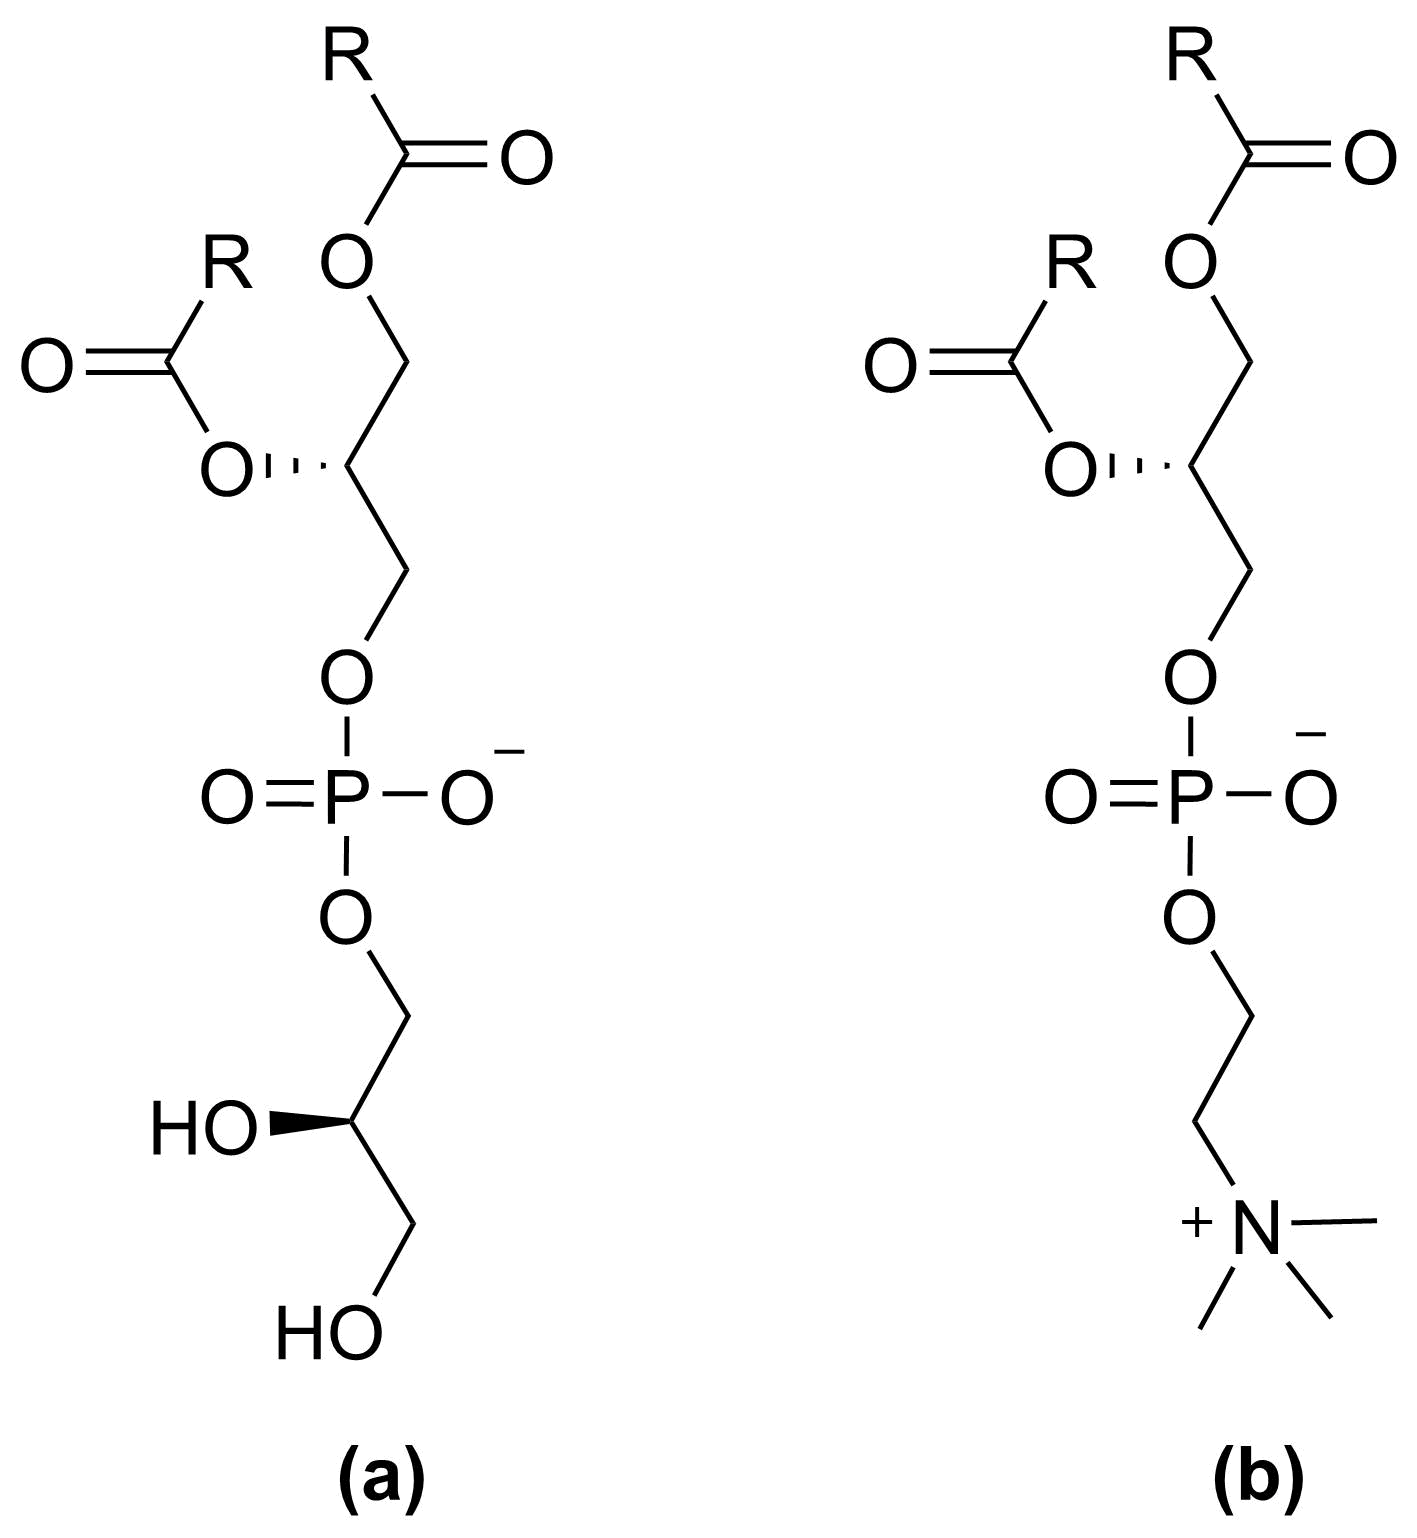
\includegraphics[width=0.30\textwidth]{figures/head_groups}
	\caption{The two lipid head groups compared in this study, where R indicates the carbon tail; (a) phosphatidylglycerol, (b) phosphocholine. Figure files are available under MIT License.\cite{mccluskey_2018}}
	\label{fig:heads}
\end{figure}

Finally, previous work has suggested that the DES may provide a segregated environment to better solubilise phospholipid head groups.\cite{Bryant2016,Bryant2017}. Since both the phosphatidylglycerol and phosphocholine head groups contain a moeity of the DES solvent, it is possible for the choline terminal of the phosphocholine would favour the presence of glycerol, while the glycerol terminal of the phosphatidylglycerol would be favourably solubilised by the choline moeity of the DES. This solvent segregation of the DES may result in the phosphocholine head group being preferentially solubilised due to the greater molar abundence of glycerol in the 1:2 mixture, and hence giving a smaller volume for this head group than found in water.

\section{Conclusions}
Stable phosphocholine and phosphatidylglycerol lipid monolayers have been observed to at the air-DES interface, and chemically-relevant modelling was used to analyse X-ray reflectometry measurements quantifying the effect that the non-aqueous solvent on the volume occupied by the head group of each lipid. The structure of the tail regions were similar to those previously found at the air-water interface, while there was clear decrease in the volume occupied by the phosphocholine head group. This decrease was not also found in the phosphatidylglycerol head group volume. 

A possible cause for this volume reduction may be the screening of the positive charge on the ammonium moeity of the phosphocholine, as this is a differential feature of the two lipid head groups. It appears that specific ion-ion interactions between the positively charged nitrogen and, most likely, the negatively charged chloride ion results in a modification to the head group charge density in DES compared to that in water. It is possible that the change observed to the head groups may be observed structurally, however insufficient instrument resolution did not allow for the precise identification of such changes. 

The ability to determine the head group volume was facilitated by access to easy to use, and open-source software that allowed for the straightforward use a custom, chemically-relevant model to be used within the analysis of the X-ray reflectometry measurements. Futhermore, this work presents the first, to our knowledge, use of chemically-relevant parameterisation to ce-refine X-ray reflectometry measurements at different surface concentrations. 

Until the emergence of ionic liquids and DES, only a limited number of molecular solvents exhibited the ability to promote self-assembly and, to the best of our knowledge, only water among those had demonstrated the formation of functional phospholipid monolayers at the air-liquid interface. Therefore, choline chloride:glycerol DES constitutes a novel environment where phospholipid membranes may be investigated. These possibilities include fundamental investigations of phospholipid monolayers in extreme environments (total or partial absence of water, cryogenic temperatures), protein membrane interactions and development of new technologies for drug delivery.

\section*{Conflicts of interest}
There are no conflicts to declare.

\section*{Acknowledgements}
The authors would like to thank the European Spallation Source and the University of Bath Alumni Fund for supporting A.S.-F. A.R.M. is grateful to the university of Bath and Diamond Light Source for co-funding a studentship (Studentship Number STU0149). We also thank Diamond Light Source and Institute Laue-Langevin for the awarded beamtime (SI10546-1 and 9-13-612 respectively).

%%%END OF MAIN TEXT%%%

%The \balance command can be used to balance the columns on the final page if desired. It should be placed anywhere within the first column of the last page.

\balance

%If notes are included in your references you can change the title from 'References' to 'Notes and references' using the following command:
%\renewcommand\refname{Notes and references}

%%%REFERENCES%%%
\bibliography{rsc} %You need to replace "rsc" on this line with the name of your .bib file
\bibliographystyle{rsc} %the RSC's .bst file

\end{document}
